
%% bare\_jrnl.tex
%% V1.3
%% 2007/01/11
%% by Michael Shell
%% see http://www.michaelshell.org/
%% for current contact information.
%%
%% This is a skeleton file demonstrating the use of IEEEtran.cls
%% (requires IEEEtran.cls version 1.7 or later) with an IEEE journal paper.
%%
%% Support sites:
%% http://www.michaelshell.org/tex/ieeetran/
%% http://www.ctan.org/tex-archive/macros/latex/contrib/IEEEtran/
%% and
%% http://www.ieee.org/



% *** Authors should verify (and, if needed, correct) their LaTeX system  ***
% *** with the testflow diagnostic prior to trusting their LaTeX platform ***
% *** with production work. IEEE's font choices can trigger bugs that do  ***
% *** not appear when using other class files.                            ***
% The testflow support page is at:
% http://www.michaelshell.org/tex/testflow/


%%*************************************************************************
%% Legal Notice:
%% This code is offered as-is without any warranty either expressed or
%% implied; without even the implied warranty of MERCHANTABILITY or
%% FITNESS FOR A PARTICULAR PURPOSE! 
%% User assumes all risk.
%% In no event shall IEEE or any contributor to this code be liable for
%% any damages or losses, including, but not limited to, incidental,
%% consequential, or any other damages, resulting from the use or misuse
%% of any information contained here.
%%
%% All comments are the opinions of their respective authors and are not
%% necessarily endorsed by the IEEE.
%%
%% This work is distributed under the LaTeX Project Public License (LPPL)
%% ( http://www.latex-project.org/ ) version 1.3, and may be freely used,
%% distributed and modified. A copy of the LPPL, version 1.3, is included
%% in the base LaTeX documentation of all distributions of LaTeX released
%% 2003/12/01 or later.
%% Retain all contribution notices and credits.
%% ** Modified files should be clearly indicated as such, including  **
%% ** renaming them and changing author support contact information. **
%%
%% File list of work: IEEEtran.cls, IEEEtran\_HOWTO.pdf, bare\_adv.tex,
%%                    bare\_conf.tex, bare\_jrnl.tex, bare\_jrnl\_compsoc.tex
%%*************************************************************************

% Note that the a4paper option is mainly intended so that authors in
% countries using A4 can easily print to A4 and see how their papers will
% look in print - the typesetting of the document will not typically be
% affected with changes in paper size (but the bottom and side margins will).
% Use the testflow package mentioned above to verify correct handling of
% both paper sizes by the user's LaTeX system.
%
% Also note that the "draftcls" or "draftclsnofoot", not "draft", option
% should be used if it is desired that the figures are to be displayed in
% draft mode.
%
\documentclass[article]{IEEEtran}

\usepackage[pdftex]{graphicx}

%diretório das figuras
\graphicspath{../pictures/} 

\usepackage{latexsym} % Símbolos
\usepackage{amsmath} % Pacoetes para matem\'iticas
\usepackage{amssymb} % Pacotes para Símbolos matem\'iticos

%\usepackage[latin1]{inputenc}
%\usepackage[brazil]{babel}

%\usepackage{multirow}
%
% If IEEEtran.cls has not been installed into the LaTeX system files,
% manually specify the path to it like:
% \documentclass[journal]{../sty/IEEEtran}





% Some very useful LaTeX packages include:
% (uncomment the ones you want to load)


% *** MISC UTILITY PACKAGES ***
%
%\usepackage{ifpdf}
% Heiko Oberdiek's ifpdf.sty is very useful if you need conditional
% compilation based on whether the output is pdf or dvi.
% usage:
% \ifpdf
%   % pdf code
% \else
%   % dvi code
% \fi
% The latest version of ifpdf.sty can be obtained from:
% http://www.ctan.org/tex-archive/macros/latex/contrib/oberdiek/
% Also, note that IEEEtran.cls V1.7 and later provides a builtin
% \ifCLASSINFOpdf conditional that works the same way.
% When switching from latex to pdflatex and vice-versa, the compiler may
% have to be run twice to clear warning/error messages.






% *** CITATION PACKAGES ***
%
%\usepackage{cite}
% cite.sty was written by Donald Arseneau
% V1.6 and later of IEEEtran pre-defines the format of the cite.sty package
% \cite{} output to follow that of IEEE. Loading the cite package will
% result in citation numbers being automatically sorted and properly
% "compressed/ranged". e.g., [1], [9], [2], [7], [5], [6] without using
% cite.sty will become [1], [2], [5]--[7], [9] using cite.sty. cite.sty's
% \cite will automatically add leading space, if needed. Use cite.sty's
% noadjust option (cite.sty V3.8 and later) if you want to turn this off.
% cite.sty is already installed on most LaTeX systems. Be sure and use
% version 4.0 (2003-05-27) and later if using hyperref.sty. cite.sty does
% not currently provide for hyperlinked citations.
% The latest version can be obtained at:
% http://www.ctan.org/tex-archive/macros/latex/contrib/cite/
% The documentation is contained in the cite.sty file itself.






% *** GRAPHICS RELATED PACKAGES ***
%
\ifCLASSINFOpdf
  % \usepackage[pdftex]{graphicx}
  % declare the path(s) where your graphic files are
  % \graphicspath{{../pdf/}{../jpeg/}}
  % and their extensions so you won't have to specify these with
  % every instance of \includegraphics
  % \DeclareGraphicsExtensions{.pdf,.jpeg,.png}
\else
  % or other class option (dvipsone, dvipdf, if not using dvips). graphicx
  % will default to the driver specified in the system graphics.cfg if no
  % driver is specified.
  % \usepackage[dvips]{graphicx}
  % declare the path(s) where your graphic files are
  % \graphicspath{{../eps/}}
  % and their extensions so you won't have to specify these with
  % every instance of \includegraphics
  % \DeclareGraphicsExtensions{.eps}
\fi
% graphicx was written by David Carlisle and Sebastian Rahtz. It is
% required if you want graphics, photos, etc. graphicx.sty is already
% installed on most LaTeX systems. The latest version and documentation can
% be obtained at: 
% http://www.ctan.org/tex-archive/macros/latex/required/graphics/
% Another good source of documentation is "Using Imported Graphics in
% LaTeX2e" by Keith Reckdahl which can be found as epslatex.ps or
% epslatex.pdf at: http://www.ctan.org/tex-archive/info/
%
% latex, and pdflatex in dvi mode, support graphics in encapsulated
% postscript (.eps) format. pdflatex in pdf mode supports graphics
% in .pdf, .jpeg, .png and .mps (metapost) formats. Users should ensure
% that all non-photo figures use a vector format (.eps, .pdf, .mps) and
% not a bitmapped formats (.jpeg, .png). IEEE frowns on bitmapped formats
% which can result in "jaggedy"/blurry rendering of lines and letters as
% well as large increases in file sizes.
%
% You can find documentation about the pdfTeX application at:
% http://www.tug.org/applications/pdftex





% *** MATH PACKAGES ***
%
%\usepackage[cmex10]{amsmath}
% A popular package from the American Mathematical Society that provides
% many useful and powerful commands for dealing with mathematics. If using
% it, be sure to load this package with the cmex10 option to ensure that
% only type 1 fonts will utilized at all point sizes. Without this option,
% it is possible that some math symbols, particularly those within
% footnotes, will be rendered in bitmap form which will result in a
% document that can not be IEEE Xplore compliant!
%
% Also, note that the amsmath package sets \interdisplaylinepenalty to 10000
% thus preventing page breaks from occurring within multiline equations. Use:
%\interdisplaylinepenalty=2500
% after loading amsmath to restore such page breaks as IEEEtran.cls normally
% does. amsmath.sty is already installed on most LaTeX systems. The latest
% version and documentation can be obtained at:
% http://www.ctan.org/tex-archive/macros/latex/required/amslatex/math/





% *** SPECIALIZED LIST PACKAGES ***
%
%\usepackage{algorithmic}
% algorithmic.sty was written by Peter Williams and Rogerio Brito.
% This package provides an algorithmic environment fo describing algorithms.
% You can use the algorithmic environment in-text or within a figure
% environment to provide for a floating algorithm. Do NOT use the algorithm
% floating environment provided by algorithm.sty (by the same authors) or
% algorithm2e.sty (by Christophe Fiorio) as IEEE does not use dedicated
% algorithm float types and packages that provide these will not provide
% correct IEEE style captions. The latest version and documentation of
% algorithmic.sty can be obtained at:
% http://www.ctan.org/tex-archive/macros/latex/contrib/algorithms/
% There is also a support site at:
% http://algorithms.berlios.de/index.html
% Also of interest may be the (relatively newer and more customizable)
% algorithmicx.sty package by Szasz Janos:
% http://www.ctan.org/tex-archive/macros/latex/contrib/algorithmicx/




% *** ALIGNMENT PACKAGES ***
%
%\usepackage{array}
% Frank Mittelbach's and David Carlisle's array.sty patches and improves
% the standard LaTeX2e array and tabular environments to provide better
% appearance and additional user controls. As the default LaTeX2e table
% generation code is lacking to the point of almost being broken with
% respect to the quality of the end results, all users are strongly
% advised to use an enhanced (at the very least that provided by array.sty)
% set of table tools. array.sty is already installed on most systems. The
% latest version and documentation can be obtained at:
% http://www.ctan.org/tex-archive/macros/latex/required/tools/


%\usepackage{mdwmath}
%\usepackage{mdwtab}
% Also highly recommended is Mark Wooding's extremely powerful MDW tools,
% especially mdwmath.sty and mdwtab.sty which are used to format equations
% and tables, respectively. The MDWtools set is already installed on most
% LaTeX systems. The lastest version and documentation is available at:
% http://www.ctan.org/tex-archive/macros/latex/contrib/mdwtools/


% IEEEtran contains the IEEEeqnarray family of commands that can be used to
% generate multiline equations as well as matrices, tables, etc., of high
% quality.


%\usepackage{eqparbox}
% Also of notable interest is Scott Pakin's eqparbox package for creating
% (automatically sized) equal width boxes - aka "natural width parboxes".
% Available at:
% http://www.ctan.org/tex-archive/macros/latex/contrib/eqparbox/





% *** SUBFIGURE PACKAGES ***
%\usepackage[tight,footnotesize]{subfigure}
% subfigure.sty was written by Steven Douglas Cochran. This package makes it
% easy to put subfigures in your figures. e.g., "Figure 1a and 1b". For IEEE
% work, it is a good idea to load it with the tight package option to reduce
% the amount of white space around the subfigures. subfigure.sty is already
% installed on most LaTeX systems. The latest version and documentation can
% be obtained at:
% http://www.ctan.org/tex-archive/obsolete/macros/latex/contrib/subfigure/
% subfigure.sty has been superceeded by subfig.sty.



%\usepackage[caption=false]{caption}
%\usepackage[font=footnotesize]{subfig}
% subfig.sty, also written by Steven Douglas Cochran, is the modern
% replacement for subfigure.sty. However, subfig.sty requires and
% automatically loads Axel Sommerfeldt's caption.sty which will override
% IEEEtran.cls handling of captions and this will result in nonIEEE style
% figure/table captions. To prevent this problem, be sure and preload
% caption.sty with its "caption=false" package option. This is will preserve
% IEEEtran.cls handing of captions. Version 1.3 (2005/06/28) and later 
% (recommended due to many improvements over 1.2) of subfig.sty supports
% the caption=false option directly:
%\usepackage[caption=false,font=footnotesize]{subfig}
%
% The latest version and documentation can be obtained at:
% http://www.ctan.org/tex-archive/macros/latex/contrib/subfig/
% The latest version and documentation of caption.sty can be obtained at:
% http://www.ctan.org/tex-archive/macros/latex/contrib/caption/




% *** FLOAT PACKAGES ***
%
%\usepackage{fixltx2e}
% fixltx2e, the successor to the earlier fix2col.sty, was written by
% Frank Mittelbach and David Carlisle. This package corrects a few problems
% in the LaTeX2e kernel, the most notable of which is that in current
% LaTeX2e releases, the ordering of single and double column floats is not
% guaranteed to be preserved. Thus, an unpatched LaTeX2e can allow a
% single column figure to be placed prior to an earlier double column
% figure. The latest version and documentation can be found at:
% http://www.ctan.org/tex-archive/macros/latex/base/



%\usepackage{stfloats}
% stfloats.sty was written by Sigitas Tolusis. This package gives LaTeX2e
% the ability to do double column floats at the bottom of the page as well
% as the top. (e.g., "\begin{figure*}[!b]" is not normally possible in
% LaTeX2e). It also provides a command:
%\fnbelowfloat
% to enable the placement of footnotes below bottom floats (the standard
% LaTeX2e kernel puts them above bottom floats). This is an invasive package
% which rewrites many portions of the LaTeX2e float routines. It may not work
% with other packages that modify the LaTeX2e float routines. The latest
% version and documentation can be obtained at:
% http://www.ctan.org/tex-archive/macros/latex/contrib/sttools/
% Documentation is contained in the stfloats.sty comments as well as in the
% presfull.pdf file. Do not use the stfloats baselinefloat ability as IEEE
% does not allow \baselineskip to stretch. Authors submitting work to the
% IEEE should note that IEEE rarely uses double column equations and
% that authors should try to avoid such use. Do not be tempted to use the
% cuted.sty or midfloat.sty packages (also by Sigitas Tolusis) as IEEE does
% not format its papers in such ways.


%\ifCLASSOPTIONcaptionsoff
%  \usepackage[nomarkers]{endfloat}
% \let\MYoriglatexcaption\caption
% \renewcommand{\caption}[2][\relax]{\MYoriglatexcaption[#2]{#2}}
%\fi
% endfloat.sty was written by James Darrell McCauley and Jeff Goldberg.
% This package may be useful when used in conjunction with IEEEtran.cls'
% captionsoff option. Some IEEE journals/societies require that submissions
% have lists of figures/tables at the end of the paper and that
% figures/tables without any captions are placed on a page by themselves at
% the end of the document. If needed, the draftcls IEEEtran class option or
% \CLASSINPUTbaselinestretch interface can be used to increase the line
% spacing as well. Be sure and use the nomarkers option of endfloat to
% prevent endfloat from "marking" where the figures would have been placed
% in the text. The two hack lines of code above are a slight modification of
% that suggested by in the endfloat docs (section 8.3.1) to ensure that
% the full captions always appear in the list of figures/tables - even if
% the user used the short optional argument of \caption[]{}.
% IEEE papers do not typically make use of \caption[]'s optional argument,
% so this should not be an issue. A similar trick can be used to disable
% captions of packages such as subfig.sty that lack options to turn off
% the subcaptions:
% For subfig.sty:
% \let\MYorigsubfloat\subfloat
% \renewcommand{\subfloat}[2][\relax]{\MYorigsubfloat[]{#2}}
% For subfigure.sty:
% \let\MYorigsubfigure\subfigure
% \renewcommand{\subfigure}[2][\relax]{\MYorigsubfigure[]{#2}}
% However, the above trick will not work if both optional arguments of
% the \subfloat/subfig command are used. Furthermore, there needs to be a
% description of each subfigure *somewhere* and endfloat does not add
% subfigure captions to its list of figures. Thus, the best approach is to
% avoid the use of subfigure captions (many IEEE journals avoid them anyway)
% and instead reference/explain all the subfigures within the main caption.
% The latest version of endfloat.sty and its documentation can obtained at:
% http://www.ctan.org/tex-archive/macros/latex/contrib/endfloat/
%
% The IEEEtran \ifCLASSOPTIONcaptionsoff conditional can also be used
% later in the document, say, to conditionally put the References on a 
% page by themselves.





% *** PDF, URL AND HYPERLINK PACKAGES ***
%
%\usepackage{url}
% url.sty was written by Donald Arseneau. It provides better support for
% handling and breaking URLs. url.sty is already installed on most LaTeX
% systems. The latest version can be obtained at:
% http://www.ctan.org/tex-archive/macros/latex/contrib/misc/
% Read the url.sty source comments for usage information. Basically,
% \url{my\_url\_here}.





% *** Do not adjust lengths that control margins, column widths, etc. ***
% *** Do not use packages that alter fonts (such as pslatex).         ***
% There should be no need to do such things with IEEEtran.cls V1.6 and later.
% (Unless specifically asked to do so by the journal or conference you plan
% to submit to, of course. )


% correct bad hyphenation here
\begin{document}
%
% paper title
% can use linebreaks \\ within to get better formatting as desired

\title{Tegra 3}

\author{Danilo Souza, Hugo Santos, Welton Ara\'ujo

\thanks{Engenharia da Computa\c{c}\~ao, Universidade Federal do Par\'a, Bel\'em-PA, Brasil}
Emails: \{dhcsouza, hugoleonardoeng07, weltonmaxx007\}@gmail.com}

\maketitle

\begin{abstract}

Mobility is undoubtedly the mark of the XXI century, more and more people are using smartphones or tablets to work, to share multimedia content (videos, photos, audio), interact in social networks, entertainment, these activities are often made at the same time as synchronizing e-mail, listen to music and update social networks. One of the great challenges of manufacturers of processors for mobile devices is to combine performance with low power consumption. So, today's users can carry out their multiple tasks simultaneously, and this problem becomes even more evident when deals with high definition multimedia content, 3D gaming, faster web browsing, etc. To solve this problem, the industry of mobile devices "imported" the concept of desktop's multi processing to smartphones and tablets. This paper will show how the Tegra 3, the newest release from NVidia for mobile phones and tablets, has achieved a optimum relationship between Performance and Power Consumption besides show the importance of multi processing.

\end{abstract}

\begin{IEEEkeywords}
Tegra 3, quad-core, vSMP, multiprocessing.
\end{IEEEkeywords}

\IEEEpeerreviewmaketitle

\section{Hist\'orico}

Fundada em 1993, por Jen-Hsun Hung, Chris Malachowsky, Curtis Priem,  com o intuito de entrar para o mercado da computa\c{c}\~ao gr\'afica, a NVidia logo se tornou uma empresa consolidada no mercado e mostrou que estava disposta a investir em tecnologia para aperfei\c{c}oar cada vez mais seus produtos, tanto que fechou sua primeira parceria com a SGS-Thompson um ano ap\'os sua cria\c{c}\~ao. No ano seguinte, lan\c{c}ou seu primeiro produto, o NV1, utilizado pelo jogo “Virtual Fighters” da Sega, l\'ider do mercado de arcades na \'epoca.

Ap\'os o sucesso, a NVidia continuou com suas inova\c{c}\~oes, e em 1996 apresentou os primeiros drivers do Microsoft DirectX.
O crescimento foi t\~ao r\'apido em t\~ao pouco tempo que, em 1999, a empresa abriu seu capital e iniciou a oferta p\'ublica de a\c{c}\~oes. Neste mesmo, ano a NVidia fez um dos lan\c{c}amentos mais grandiosos da empresa, e que sem d\'uvida, revolucionou a ind\'ustra. O GPU, um processador de chip \'unico capaz de processar, na \'epoca, 10 milh\~oes de pol\'igonos por segundo, nos GPU’s mais modernos esse n\'umero chega a 2 bilh\~oes.

Atualmente a empresa atua fabricando processadores espec\'ificos para diversas \'areas como a ind\'ustria automobil\'istica, tables, smartfones, supercomputadores, etc.
Em Fevereiro de  2011 a empresa apresentou o projeto Kal-El (Tegra 3), primeiro processador quad-core do mundo criado para atender a nova demanda de aplica\c{c}\~oes para mobilidade  e melhorar a experi\^encia de aplica\c{c}\~oes j\'a existentes.

\section{Introdu\c{c}\~ao}

\'E ineg\'avel que o futuro da comuni\c{c}\~ao est\'a dentro de tablets e smartfones, cada vez mais pessoas compram estes dispositivos para se conectar à internet e realizar atividades cotidianas, como ler/enviar e-mails, ver v\'ideos, utilizar as redes sociais, e com o avan\c{c}o exponencial da internet e das pr\'oprias tecnologias relacionadas \`a multim\'idia e jogos. As exig\^encias para os tablets e smartfones aumentaram, os usu\'arios n\~ao querem mais simplesmente ler e-mail ou navegar no site do banco, o mercado hoje em dia \'e muito mais exigente, e busca cada vez mais coisas sofisticadas, como por exemplo, assistir v\'ideos em alta defini\c{c}\~ao, jogos em 3D, carregar uma p\'agina web de alta resolu\c{c}\~ao, v\'ideo confer\^encias de alta defini\c{c}\~ao em tempo real, etc.

Contudo, os processadores de prop\'osito geral utilizados na maioria dos dispositivos m\'oveis atualmente n\~ao suprem essa necessidade com a efic\^encia desejada. Visando esse mercado, a NVidia lan\c{c}ou a arquitetura Tegra, uma arquitetura heterog\^enea baseada em multi-processadores, utilizando-se de 8 processadores de prop\'osito espec\'ifico para processamento de gr\'aficos, imagens, \'audio, codifica\c{c}\~ao/decodifica\c{c}\~ao de v\'ideos, etc.

O grande desafio em lidar com as novas exig\^encias do mercado est\'a em balancear um alto desempenho com baixo consumo de energia, a melhor maneira de juntar as duas e obter uma boa rela\c{c}\~ao custo benef\'icio \'e trazer para o mundo m\'ovel o conceito de processadores com v\'arios n\'ucleos, amplamente utilizado no mundo dos desktops. Assim, \'e poss\'ivel aumentar a efici\^encia do processamento, uma vez que duas ou mais tarefas podem ser realizada ao mesmo tempo, sem ter que aumentar a frequ\^encia de clock dos processadores, o que acarretaria em um maior consumo de energia.

A NVidia lan\c{c}ou os processadores Tegra 2 e Tegra 3 (Projeto Kal-El), com 2 e 4 n\'ucleos, respectivamente, sendo que este \'ultimo possui uma enorme evolu\c{c}\~ao de desempenho quando comparado ao primeiro. Nas sess\~oes seguintes ser\~ao explicadas com mais detalhes as caracter\'isticas que permitem com que o Tegra 3 alcance uma \'otima rela\c{c}\~ao entre consumo de energia e desempenho.

\section{Caracter\'isticas}

\subsection{Multiprocessamento}

Multi-processamento \'e sem d\'uvida uma das melhores formas de obter um dispositivo com alto desempenho e baixo consumo de energia, entretanto, quanto mais n\'ucleos, maior \'e a economia de energia. Para executar uma mesma atividade, um processador com 2 n\'ucleos precisa de uma frequ\^encia de clock maior do que um processador de 4 n\'ucleos precisaria, al\'em do fato de que o processador com 2 n\'ucleos ficaria ativo por mais tempo na frequ\^encia de pico, aumentando assim o consumo de energia. 

Multi-processamento \'e sem d\'uvida uma das melhores formas de obter um dispositivo com alto desempenho e baixo consumo de energia, entretanto, quanto mais n\'ucleos, maior \'e a economia de energia. Para executar várias atividades em paralelo, um processador com 2 n\'ucleos precisa de uma frequ\^encia de clock maior do que um processador de 4 n\'ucleos precisa para obter um mesmo desempenho. As altas frequ\^encias aumentam o consumo de energia. A Figura \ref{fig:quadcorephota} mostra um comparativo entre os processadores Tegra 2 e Tegra 3, enquanto que a Figura \ref{fig:multithread} mostra um comparativo quando se utiliza 2 e 4 n\'ucleos do Tegra 3.

Dispositivos m\'oveis frequentemente executam diversas atividades ao mesmo tempo, p.e, sincroniza\c{c}\~ao de e-mail/redes sociais, navega\c{c}\~ao web, atualizador de not\'icias, etc. Se todas essas atividades fossem executadas por um \'unico n\'ucleo, este ficaria mais tempo na frequ\^enia de pico, gastando assim mais energia, al\'em de n\~ao conseguir uma resposta satisfat\'oria. As Figuras \ref{fig:quadcorebenchmark} e \ref{fig:quadcorevideo} mostram um comparativo entre processadores Quad Core e Dual Core, em rela\c{c}\~ao ao Moonbat Benchmark e codifica\c{c}\~ao de v\'ideo, respectivamente.

\begin{figure}[ht]
  \centering
  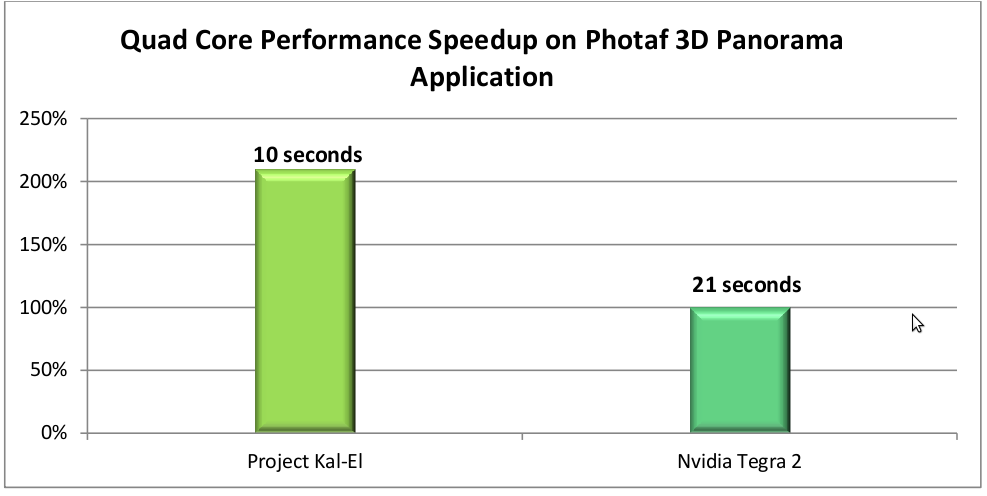
\includegraphics[width=8.5cm]{./pictures/QaudCorePhota.png}
  \caption{Comparativo de benchmark entre processadores Quad e Dual Core}
  \label{fig:quadcorephota}
\end{figure}

\begin{figure}[ht]
  \centering
  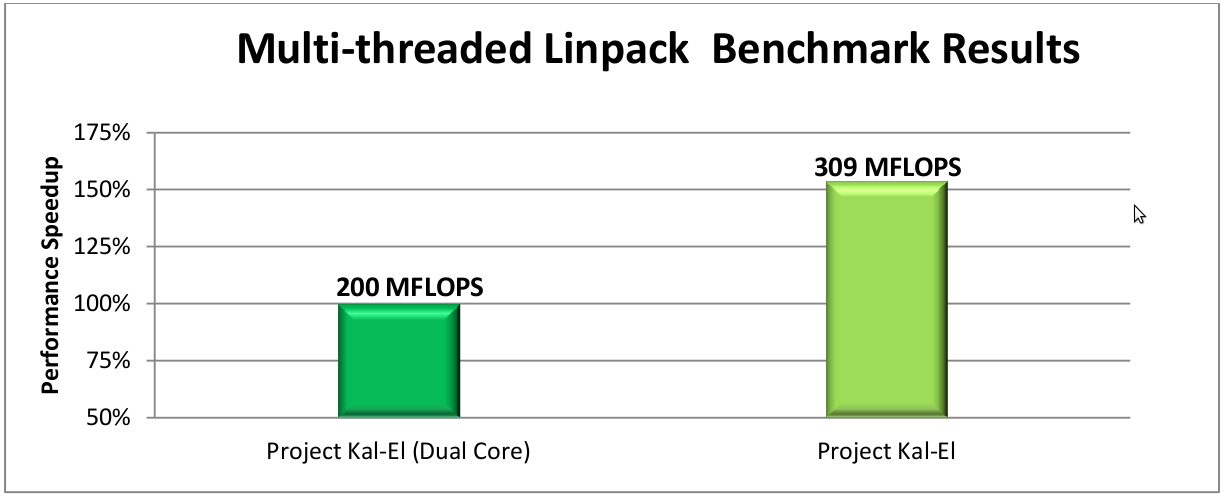
\includegraphics[width=8.5cm]{./pictures/MultiThread.png}
  \caption{Comparativo de benchmark do Tegra usando 2 e 4 n\'ucleo}
  \label{fig:multithread}
\end{figure}

\begin{figure}[ht]
  \centering
  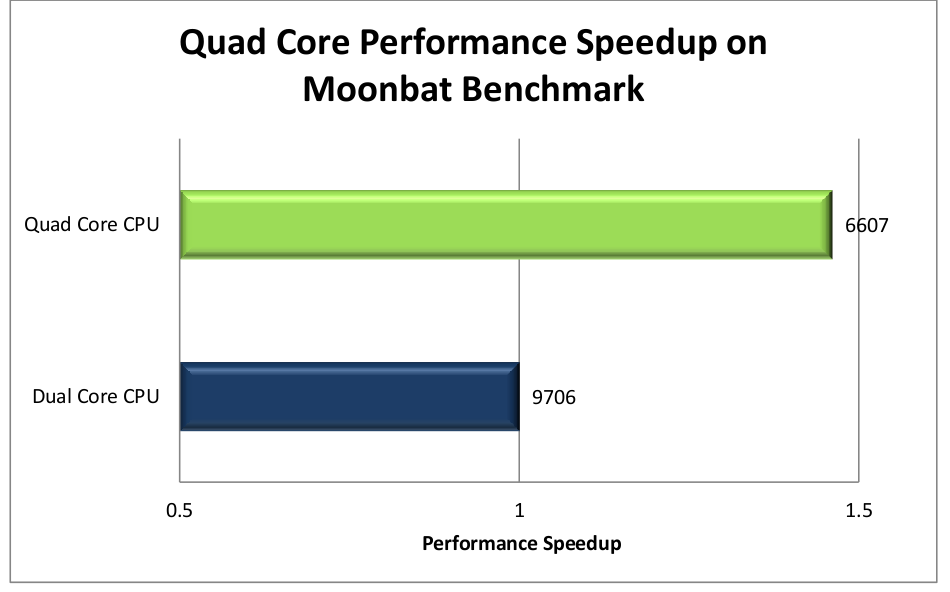
\includegraphics[width=8.5cm]{./pictures/QuadCoreBenchmark.png}
  \caption{Comparativo de benchmark entre processadores Quad e Dual Core}
  \label{fig:quadcorebenchmark}
\end{figure}

\begin{figure}[ht]
  \centering
  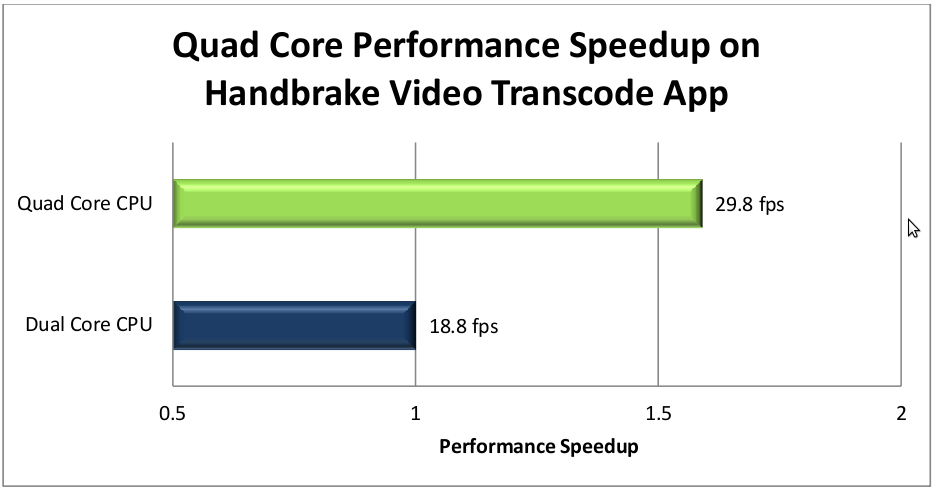
\includegraphics[width=8.5cm]{./pictures/QuadCoreVideo.png}
  \caption{Comparativo de codifica\c{c}\~ao de v\'ideo entre processadores Quad e Dual Core}
  \label{fig:quadcorevideo}
\end{figure}

\subsection{Processo de fabrica\c{c}\~ao do dispositivo de Sil\'icio X Consumo de Energia}

A tecnologia usada no processo de fabrica\c{c}\~ao de um dispositivo de sil\'ico influencia diretamente no consumo de energia uma vez que o consumo total de um dispositivo de sil\'icio \'e dado pela soma da energia de fuga (Leakage Power) e da energia din\^amica (Dynamic Power), sendo esta primeira diretamente influenciada pela tecnologia utilizada no processo. A segunda depende principalmente da frequ\^encia e pelo quadrado das tens\~oes de opera\c{c}\~ao do dispositivo. Se convencionarmos Energia Din\^amia = ED, Energia de Fuga = EF, Energia Total = ET, frequ\^encia = f (clock) e tens\~ao = V, temos que:
 
\( ET\ =\ EF\ +\ ED \)

\( ED\  \alpha\  fV^2\)
	
A partir destas defini\c{c}\~oes \'e poss\'ivel concluir que quanto mais perto da frequ\^encia de pico o dispositivo opera, mais a ET depende somente da ED, enquanto que, quanto menor a  frequ\^encia, mais a ET depende somente da EF.

Existem duas tecnologias diferentes para se construir transistores usados nos processadores. A primeira \'e a tecnologia de processo r\'apido (Fast Process Technology), que consome uma maior EV, contudo, possuem um tempo de troca muito curto quando opera em tens\~oes normais. A segunda \'e a tecnologia de processo de baixa pot\^encia (Low Power Process Technology) consome menor EF, entretanto possui um tempo maior de troca operando em tens\~oes normais.

N\'ucleos constru\'idos utilizando a primeira tecnologia possuem um maior consumo de EF, entretanto n\~ao necessitam de um grande aumento de tens\~ao quando passam a operar em frequ\^encias maiores, no caso do Tegra 3 acima de 500 MHz, e os n\'ucleos constru\'idos utilizando a segunda tecnologia  possuem menor EF, por\'em precisam de um grande aumento de tens\~ao quando passam a operar em frequ\^encias mais altas. Em resumo:

\begin{itemize}
 \item Processo r\'apido: Otimizado para altas frequ\^encias, contudo maior EF.
 \item Processo de baixa pot\^encia: Feito para operar a baixas frequ\^encias, por\'em menor EF.
\end{itemize}  

A Figura \ref{fig:tecnologiaprocesso} mostra um comparativo entre as duas tecnologias.

\begin{figure}[ht]
  \centering
  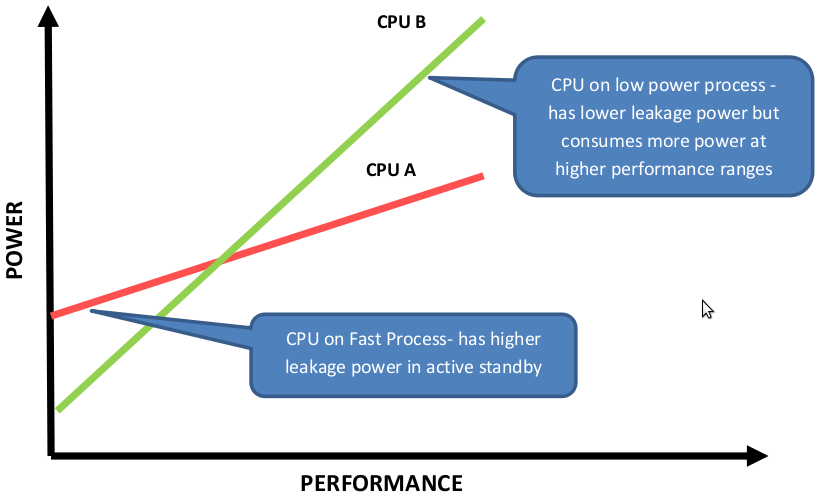
\includegraphics[width=8.5cm]{./pictures/Tecnologiasdeprocesso.png}
  \caption{Comparativo entre as diferentes tecnologias de fabrica\c{c}\~ao de chips de Sil\'icio}
  \label{fig:tecnologiaprocesso}
\end{figure}

\subsection{vSMP}

Implementada inicialmente no Projeto Kal-El, a tecnologia de Multi processamento Sim\'etrico Vari\'avel, vSMP(Variable Symmetric Multiprocessing), \'e, junto com a tecnologia de processo r\'apido para constru\c{c}\~ao dos 4 n\'ucleos principais, a principal caracter\'istica respons\'avel por reduzir dr\'asticamente o consumo de energia no Tegra 3. Ela consiste na adi\c{c}\~ao de um quinto n\'ucleo, fabricado utilizando a tecnologia de processo de baixa pot\^encia, utilizado para executar tarefas em segundo plano (sincroniza\c{c}\~ao de e-mail/redes sociais, tocar m\'usica, etc.). Esse n\'ucleo, chamado de Companion Core alcan\c{c}a uma frequ\^encia m\'axima de clock de 500 MHz.

Utilizando essa combina\c{c}\~ao de tecnologias e arquiteturas, a tecnologia vSMP \'e capaz de obter um baixo consumo ao realizar tarefas secund\'arias (baixa frequ\^encia), mas tamb\'em \'e capaz de operar a altas frequ\^encias sem necessitar de um ganho significativo na ED. A Figura \ref{fig:companiocore} mostra a arquitetura utilizando o Companion Core e a Figura \ref{fig:vsmp} mostra a combina\c{c}\~ao que resulta na tecnologia vSMP.

\begin{figure}[ht]
  \centering
  \includegraphics[width=8.5cm]{./pictures/CompanionCore.pdf}
  \caption{Arquitetura do Tegra 3 com o Companio Core}
  \label{fig:companiocore}
\end{figure}

\begin{figure}[ht]
  \centering
  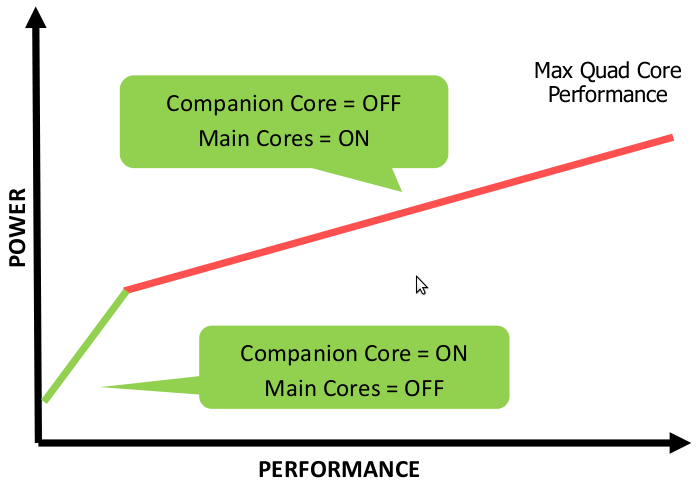
\includegraphics[width=8.5cm]{./pictures/vSMP.png}
  \caption{Compartamento das duas tecnologias de fabrica\c{c}\~ao de chips de sil\'icio combinadas}
  \label{fig:vsmp}
\end{figure}

Abaixo as principais vantagens da Arquitetura vSMP:

\begin{itemize}
 \item Transpar\^encia para o Sistema Operacional (SO)

A partir da vers\~ao 3.0 (Honey Comb) o Android oferece suporte nativo para multi processamento, sendo assim capaz de se beneficiar das vantagens de processadores com dois ou mais n\'ucleos, apesar de que, para o SO, todos os n\'ucleos possuem a mesma capacidade perform\'atica. O projeto Kal-El implementa gerenciamento baseado em hardware e linguagens de baixo n\'ivel tanto para os 4 n\'ucleos principais quanto para o Companion Core.

Esse monitoramento, utilizando software e hardware propriet\'arios, \'e respons\'avel por verificar a carga de trabalho da CPU. Dependendo dessa carga de trabalho e das recomenda\c{c}\~oes da frequ\^encia de opera\c{c}\~ao feitas pelo sistema de controle de frequ\^encia da CPU, do Kernel, esse software sinaliza para o hardware quando realizar a troca entre os n\'ucleos principais e o Companion Core. Esse procedimento \'e 100\% implementado no Tegra 3, ou seja, n\~ao requer nenhuma altera\c{c}\~ao no SO, fazendo com que esta tecnologia seja totalmente vi\'avel do ponto de vista econ\^omico.

\item Coer\^encia de Mem\'oria Cache

Quando se lida com processadores com frequ\^encia de clock diferentes, a sincroniza\c{c}\~ao de mem\'oria cache pode ser um grande problema, pois quando um processador de frequ\^encia mais baixa fizer uma opera\c{c}\~ao de escrita na mem\'oria, pode n\~ao haver tempo suficiente para que todas as mem\'orias sejam sincronizadas, o que ocasionaria um erro de leitura dos processadores de frequ\^encia mais alta. A arquitetura vSMP evita isso, simplesmente n\~ao permitindo que os n\'ucleos principais e o Companion Core estejam habilitados ao mesmo tempo, uma vez que eles compartilham a mesma mem\'oria cache de n\'ivel 2.

A Figura \ref{fig:powersavesvsmp} mostra a efici\^encia da arquitetura vSMP quanto ao consumo de energia, em compara\c{c}\~ao com seu antecessor Tegra 2, para determinadas tarefas. A Tabela \ref{tab:table1} mostra a rela\c{c}\~ao Consumo X Performance do projeto Kal-El comparado com seus concorrentes dual-core. As Figuras \ref{fig:kalellowerfrequency} e \ref{fig:kalelhigherfrequency} mostram a representa\c{c}\~ao gr\'afica da Tabela \ref{tab:table1}.

\end{itemize}

\begin{table}[ht]
  \centering
  \caption{Comparativo de consumo de energia entre concorrentes}
  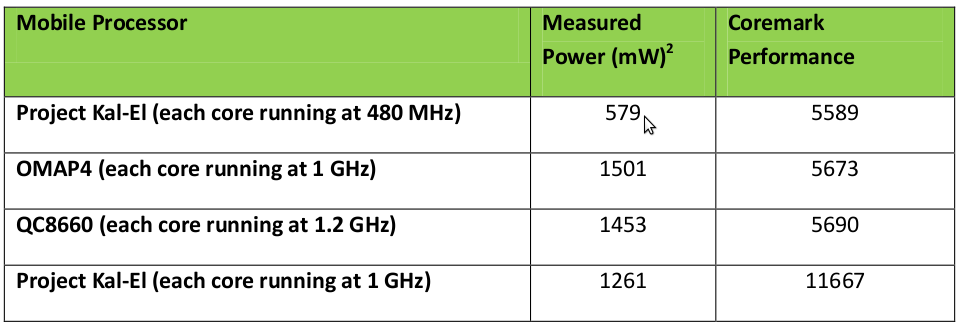
\includegraphics[width=8.5cm]{./pictures/Table1.png}
  \label{tab:table1}
\end{table}

\begin{figure}[ht]
  \centering
  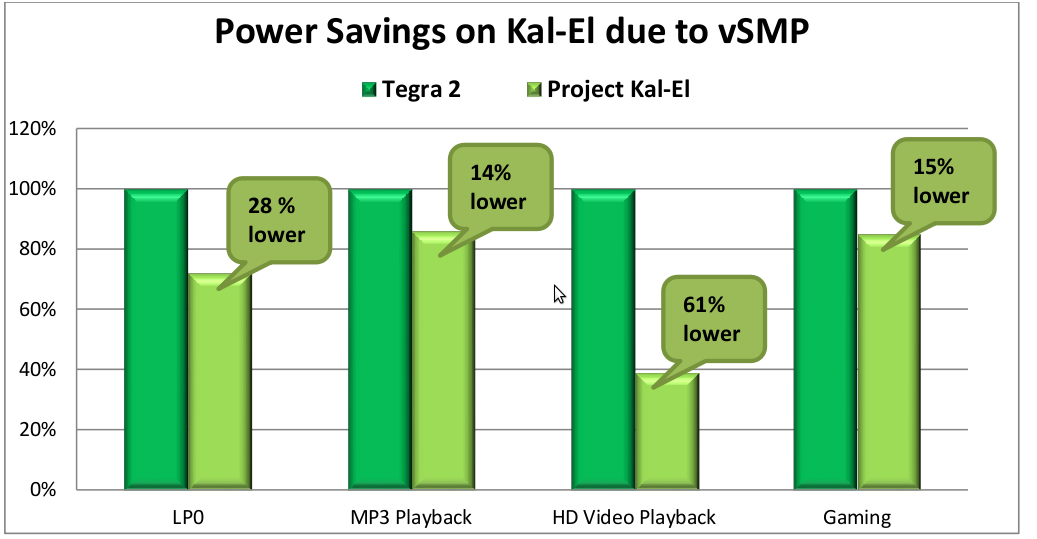
\includegraphics[width=8.5cm]{./pictures/PowerSavesVSMP.png}
  \caption{Efici\^encia da arquitetura vSMP quanto ao consumo de energia}
  \label{fig:powersavesvsmp}
\end{figure}

\begin{figure}[ht]
  \centering
  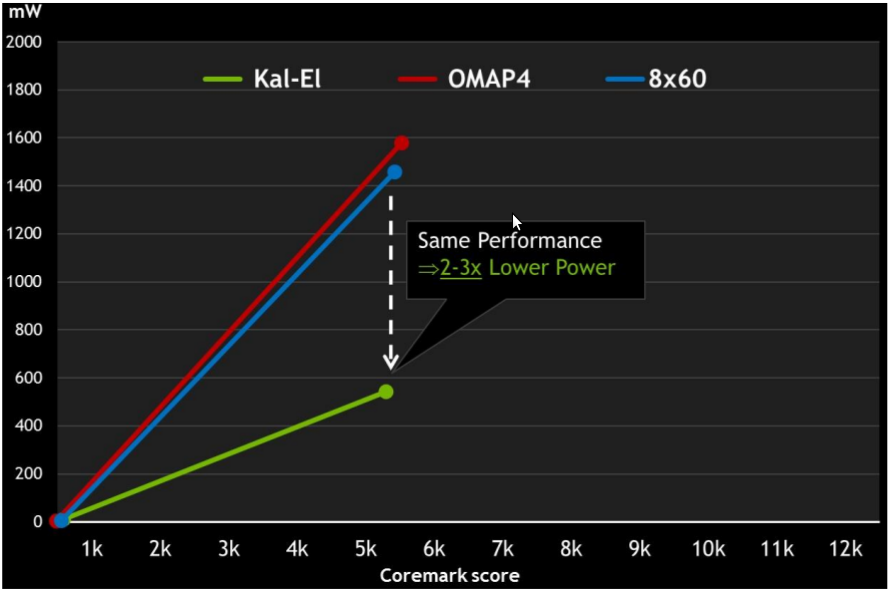
\includegraphics[width=8.5cm]{./pictures/Kal-ElLowerFrequency.png}
  \caption{Representa\c{c}\~ao gr\'afica quando cada n\'ucleo opera a 480MHz}
  \label{fig:kalellowerfrequency}
\end{figure}

\begin{figure}[ht]
  \centering
  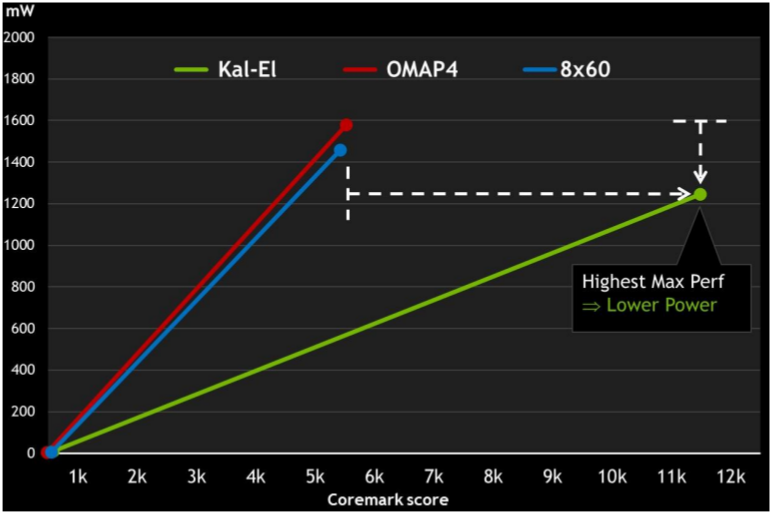
\includegraphics[width=8.5cm]{./pictures/Kal-ElHigherFrequency.png}
  \caption{Representa\c{c}\~ao gr\'afica quando cada n\'ucleo opera a 1GHz}
  \label{fig:kalelhigherfrequency}
\end{figure}

\section{Conclus\~ao}
Com o mercado cada vez mais competitivo, as empresas t\^em que buscar solu\c{c}\~oes inovadores e cada vez mais atreladas ao baixo consumo de energia e ao desempenho. Uma vez que as aplica\c{c}\~oes est\~ao ficando mais exigentes do ponto de vista computacional e a exig\^encia uma maior e mais r\'ipida intera\c{c}\~ao com as aplica\c{c}\~oes pelos usu\'arios.

Ap\'os a an\'alise dos gr\'aficos de desempenho, \'e possível perceber uma tend\^encia no aumento do n\'umero de n\'ucleos dos processadores, por\'em n\~ao basta aumentar demasiadamente o n\'umero de n\'ucleossem construir uma arquitetura otimizada para o uso desses n\'ucleos.

\ifCLASSOPTIONcaptionsoff
\newpage
\fi



\begin{thebibliography}{eu}

%\bibitem{IEEEhowto:kopka}
%H.~Kopka and P.~W. Daly, \emph{A Guide to \LaTeX}, 3rd~ed.\hskip 1em plus
%  0.5em minus 0.4em\relax Harlow, England: Addison-Wesley, 1999.

\bibitem{multicores:whitepaper}
http://www.nvidia.com/content/PDF/tegra\_white\_papers/Benefits-of-Multi-core-CPUs-in-Mobile-Devices\_Ver1.2.pdf

\bibitem{quadcore:whitepaper}
http://www.nvidia.com.br/content/PDF/tegra\_white\_papers/tegra-whitepaper-0911a.pdf

\bibitem{vSMP:whitpaper}
http://www.nvidia.com/content/PDF/tegra\_white\_papers/Variable-SMP-A-Multi-Core-CPU-Architecture-for-Low-Power-and-High-Performance.pdf

\end{thebibliography}

\end{document}
